\documentclass[12pt]{article}
\usepackage[frenchb]{babel}
\usepackage{fontspec}
\usepackage{amsmath}
\usepackage{amsfonts}
\usepackage{amssymb}
\usepackage{graphicx}
\usepackage{hyperref}
\usepackage{xcolor}
\usepackage{minted}
\usepackage{longtable}
\hypersetup{
	colorlinks,
	linkcolor={red!50!black},
	citecolor={blue!50!black},
	urlcolor={blue!80!black}
}
%\usepackage[left=2cm,right=2cm,top=2cm,bottom=2cm]{geometry}
\setmainfont{DejaVu Sans}
\newcommand{\tab}{    }
\renewcommand{\thesection}{\Roman{section}. }
\renewcommand{\thesubsection}{\tab\arabic{subsection}. }
\renewcommand{\thesubsubsection}{\tab\alph{subsubsection}) }
\renewcommand{\baselinestretch}{1.1}
\begin{document}
	\begin{titlepage}
		\centering
		{\scshape\LARGE Lycée René Descartes \par}
		\vspace{1cm}
		{\huge\bfseries \textit{"The Music Swagger"} :\par De la musique interactive\par}
		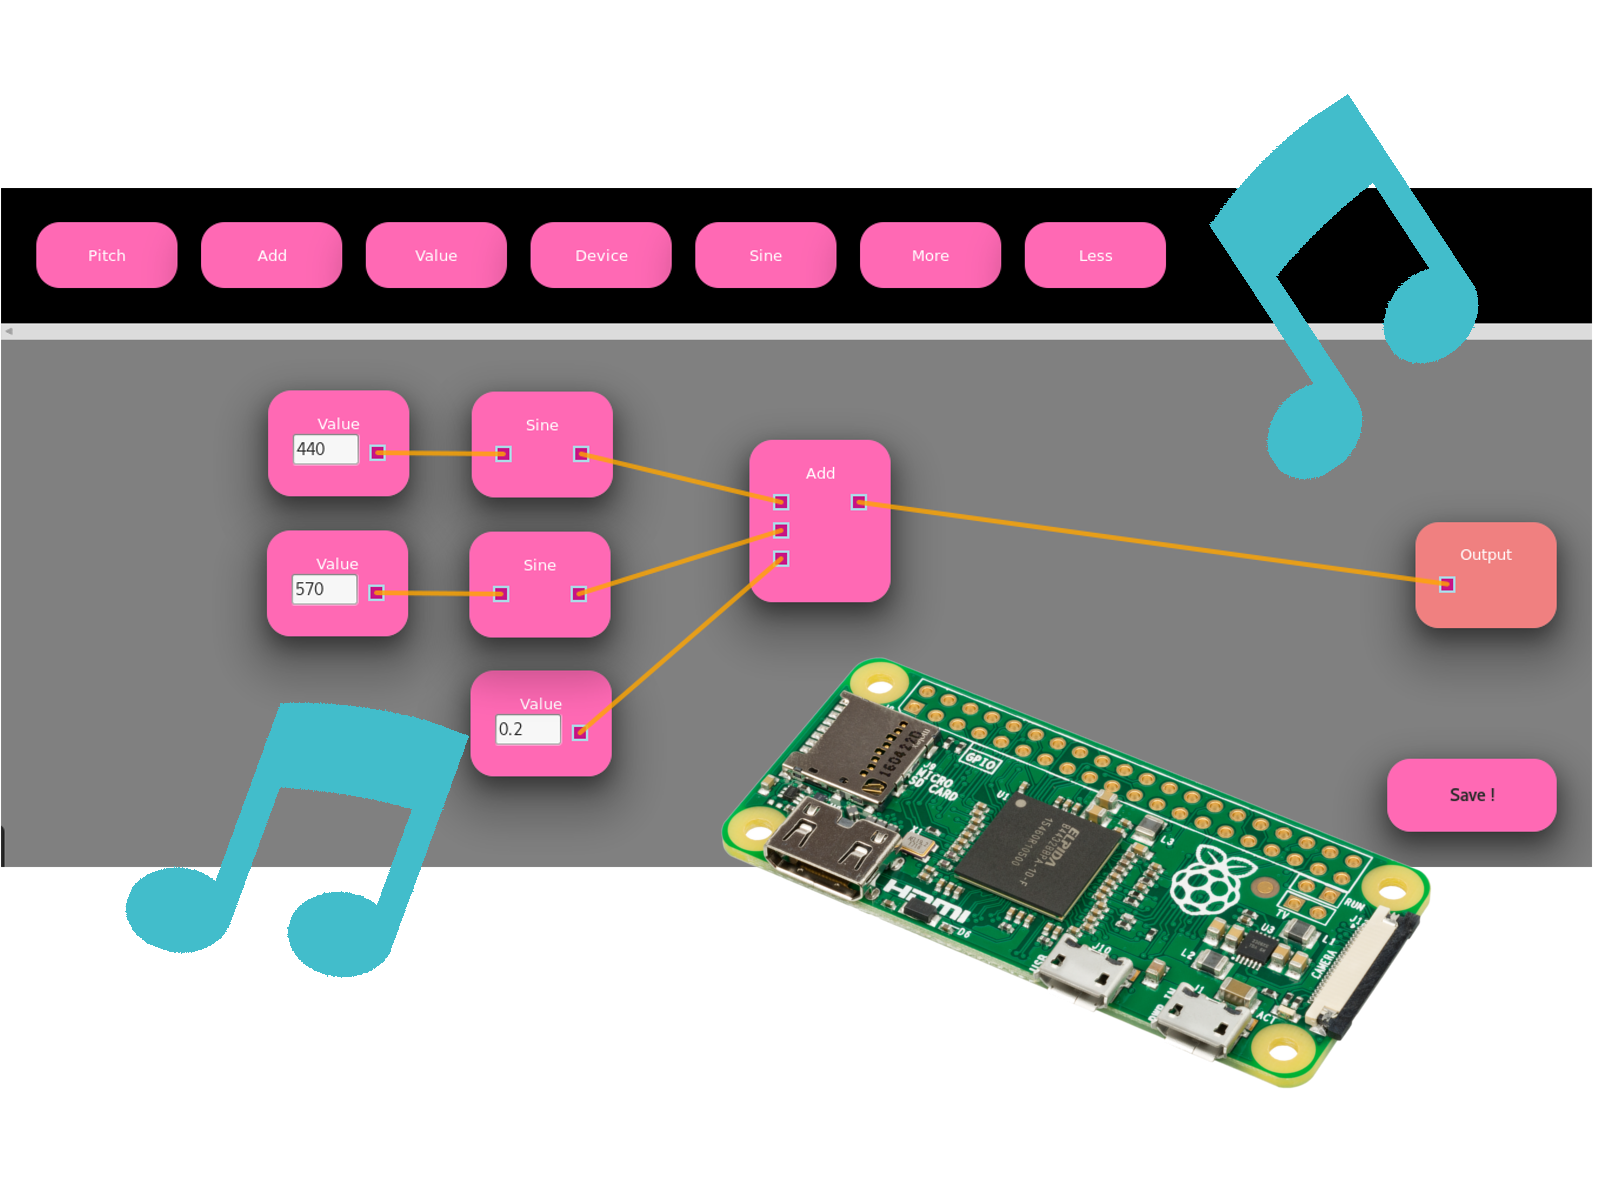
\includegraphics[height=10cm]{presentation_image}
		
		{\Large\itshape Estelle FIKET\\Thomas POTIER\\Nour BOULAHCEN\par}
		\vfill
		encadré par\par
		Mr. Bernigole
		
		\vfill
		
		{\large \today\par}
	\end{titlepage}
	\tableofcontents
	\newpage
	\section{Présentation}
	\paragraph{}
	Passionné par l'informatique, je souhaitais m'attaquer à un projet complexe réalisable en équipe. Avec Estelle et Nour, nous avions d'abord pensé à développer un jeu de type "Rogue" ou le joueur explore plusieurs niveaux. Puis, suite à nos discussions, nous avons décidé de créer un système fonctionnant comme un instrument de musique numérique : nous avons imaginé un système qui permettrait de générer du son en fonction de paramètres physiques tels que l'accélération, la distance ou tout ce qui peut être numérisé.
	\paragraph{}
	En effet, le traitement du son est un domaine qui nous plaisait  et ce projet fait appel aux différentes notions étudiées cette année en cours d'ISN : représentation de l'information, algorithmique, langage et programmation ainsi que les architectures matérielles. De plus, notre idée ne semblait pas être déjà existante ou tout du moins très peu connue.
	\paragraph{}
	C'est ainsi que nous nous sommes lancés dans "\textit{The Music Swagger}". L'idée du projet est de produire un système permettant de créer et faire varier des sons afin de générer une musique à partir de capteurs physiques (tels que gyroscope, mètres ultrasons, ou encore photodiodes). Nous avons souhaité privilégier l'ergonomie qui permet à un utilisateur non expérimenté de pourvoir simplement utiliser le projet grâce à un fonctionnement "Plug\&Play" et une interface Web simplifiée.
	
	\newpage
	\section{La mise en œuvre}
	\subsection{Les objectifs}
	\paragraph{}
	Nous nous sommes donné pour objectif de réaliser un système de génération de son à partir de données physiques. Afin d'y parvenir, nous avons avons défini plusieurs modules.
	\begin{itemize}
		\item une partie "server" qui gère la synthèse du son ainsi que l'organisation des données
		\item une partie "device" qui s'occupe de rapatrier les données d'un capteur physique (accéléromètre par exemple) au serveur
		\item une partie "client" qui permet la configuration du système
	\end{itemize}
	\paragraph{}
	La partie "server" doit permettre le stockage des données reçues des "devices" tout en gardant leur origine. Elle est elle-même composée de plusieurs sous-parties distinctes : une partie Synthèse, une partie Communication et une partie Configuration.
	\paragraph{}
	La partie "device" doit permettre un fonctionnement automatique et abstrait de capteurs : cette partie est composée d'un module de communication ainsi que d'un module de gestion du capteur. Chaque "device" doit être fonctionnel après une simple implémentation d'un capteur et une alimentation.
	\paragraph{}
	La partie "client" est basée sur une interface Web permettant une portabilité et une facilité d'utilisation. Elle doit permettre de choisir quel son sera généré à partir de quel "device" et comment. Elle doit être intuitive et elle fonctionne en "boite" "drag\&drop".
	\subsection{Les logiciels}
	\subsubsection{Outils}
	\paragraph{}
	Afin de nous aider durant la phase de programmation et de reflexion, nous avons utilisé plusieurs logiciels. Le logiciel Web \textit{Slack} (\url{slack.com}) a été choisi pour discuter et partager des morceaux de code et des idées au sein de notre groupe de travail. C'est une application permettant le "chat" ainsi que le partage de fichier et l'intégration de tierces parties comme \textit{GitHub}. \textit{Git} par le biais de \textit{GitHub} est donc le second logiciel dont nous nous sommes servis afin de partager le code, y avoir un accès constant et pouvoir connaître l'évolution du projet. Enfin, je me suis servi du logiciel \textit{PyCharm Community Edition} qui est gratuit pour un usage personnel et non commercial et qui est très puissant quand à la programmation en python notamment grâce à une correction syntaxique, orthographique (peu utile en Python mais pratique) et une correction logique (utilisation de variables qui n'existent pas, conseils d'optimisation ou d'inutilité d'une partie du code). Nous nous sommes servis d'un server \textit{L(W)AMP} (Linux (Windows) - Apache - MySQL - PHP) pour le serveur Web. J'ai travaillé tout au long du projet sur un \textit{Linux} (dérivé de \textit{Debian} plus précisément) qui je pense est le logiciel le plus adapté à la programmation. Les ordinateurs \textit{Raspberry} fonctionnent sous \textit{Raspbian Light}. La totalité des logiciels que nous avons utilisé sont gratuits même s'il ne sont pas tous open-source.
	\paragraph{}
	J'ai d'ailleurs proposé à Estelle et Nour de leur installer un système \textit{Linux} sur une clé USB afin qu'ils puissent utiliser leur ordinateur personnel et pour leur expliquer tout ce dont ils avaient besoin sur \textit{Git} et autres. C'était peut-être un peu compliqué pour eux, car après plusieurs propositions, je n'ai pas eu de clé USB de leur part. J'ai donc été le seul à publier mon code sur \textit{GitHub}.
	\subsubsection{Langages}
	\paragraph{}
	Notre projet possède une complexité qui réside dans le nombre important de langages que nous utilisons. En effet, nous avons eu besoin des languages suivant : Python3, PHP (PHP: Hypertext Preprocessor), HTML5 (HyperText Markup Language), JS (JavaScript), CSS3 (Cascading Style Sheets) et le SQL (Structured Query Language).
	
	\begin{itemize}
		\item[\textbf{Python3}] Le Python3 a été utilisé pour une grande partie du projet notamment dans la communication entre le "server" et les "devices" ainsi que dans la génération du son.
		\item[\textbf{PHP}] Le PHP nous à servi au niveau du "server" pour permettre une communication avec la base de données. 
		\item[\textbf{HTML5, JS, CSS3}] Ces languages nous ont servi dans la partie configuration du "server" pour l'interface Web. Le JS a permis l'interaction avec l'utilisateur notamment pour le "drag\&drop". Le CSS3 a servi pour l'esthétique des pages et l'HTML5 à la forme et au contenu de ces dernières.
		\item [\textbf{SQL}] Le SQL nous a permis d'interagir entre le PHP et la base de donnée MySQL.
		\item[\textbf{\LaTeX}] J'ai utilisé ce langage pour écrire mon dossier.
	\end{itemize}
	\subsubsection{Communication}
	\paragraph{}
	Afin de faire communiquer les parties entre elles, nous avons utiliser plusieurs moyens.
	\begin{itemize}
		\item[\textbf{Wi-Fi/UDP/IP}] Ce sont les protocoles utilisés pour la communication entre les "devices" et le "server".
		\item[\textbf{JSON}] C'est la façon dont nous envoyons la configuration à la page permettant de l'enregistrer via une requête "POST".
		\item[\textbf{MusicSwaggerProtocol}] C'est le protocole que nous avons inventer afin de pouvoir faire communiquer les "devices" et le "server" basé sur UDP/IP.
	\end{itemize}
	\subsubsection{Source d'information}
	\paragraph{}
	Nous avons souvent utilisé des sites internet suivants :
	\begin{itemize}
		\item[\url{http://stackoverflow.com}] pour des erreurs connues et des astuces
		\item[\url{http://developer.mozilla.org}] pour tout ce qui touche au développement Web
	\end{itemize}

	\paragraph{}
	Nous utiliserons ensuite les termes suivants : "device" pour qualifier l'ensemble Raspberry Pi et capteur, "server" pour l'ensemble serveur Web et serveur Python3.
	Pour permettre la communication entre les "devices" et le "server", nous avons opter pour un système de liaison par Wi-Fi, et des "devices" à base de Raspberry Pi Zero W pour la portabilité et le prix. Une interface Web sera mise en place afin de pouvoir configurer le comportement de façon simple et sans besoin d'application particulière. Nous avons choisis d'utiliser Python3 pour sa simplicité, sa portabilité ainsi que la richesse de ses modules. L'interface Web est composée de PHP pour l'interaction avec la base de donnée et l'HTML, JS et CSS pour la mise en forme et les interactions avec l'utilisateur (notamment avec le système de "Nodes" en "drag\&drop").
	\subsection{Le rôle de chacun}
	\noindent
	\begin{tabular}{|p{0.4\textwidth}|p{0.2\textwidth}|p{0.3\textwidth}|}
		\hline
		Taches&Planning&\\\hline
		Interface Web&≈20h&Nour, Estelle, Thomas\\
		Communication&≈10h&Thomas\\
		Device&≈10h&Thomas\\
		Server&≈10h&Thomas, Nour, Estelle\\
		Intégration&≈2h&Thomas\\
		\hline
	\end{tabular}

	\newpage
	\section{Réalisation}
	\subsection{Mon travail}
	\paragraph{}
	Voici une représentation du projet dans sa globalité.
	
	\vspace{1cm}
	\noindent
	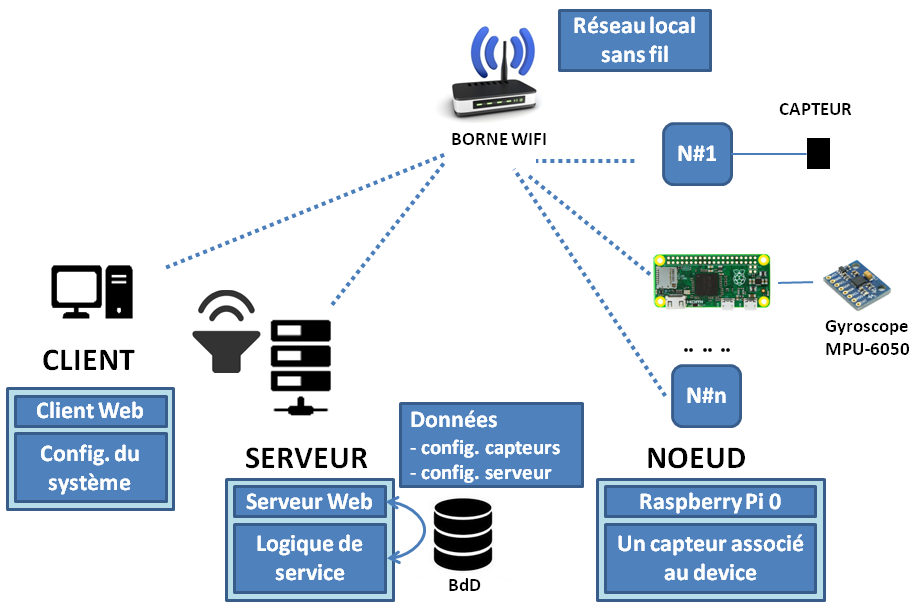
\includegraphics[width=\textwidth]{overall_sheme}
	\vspace{1cm}
	\begin{itemize}
		\item[\textbf{"device"}] C'est la partie englobant le capteur, le "DeviceBrain" et une partie de communication. Elle communique avec le "server" grâce à un "communicator" (interface de transfert de donnée par réseau (Wi-Fi) sur UDP/IP).\\
		\item[\textbf{"server"}] C'est la partie qui permet de générer le son, la réelle partie qui met en forme et concrétise le projet. Elle contient une partie de génération de son, une partie de structuration des modifications du son et d'une partie de communication avec les "devices". Elle a un accès à la base de donnée du "configurator" pour générer du son en fonction de ce que l'utilisateur désire.\\
		\item[\textbf{"configurator"}] C'est l'interface Web basé sur un serveur \textit{LAMP}, indépendante du reste du projet par ses langages (différent de Python3). Elle communique ses données à travers une base de donnée. Elle est intuitive et fonctionne par "drag\&drop" de boites et liens.
	\end{itemize}
	
	\paragraph{}
	Afin d’utiliser au mieux les compétences de chacun, il a fallu discuter de ce que chacun souhaitait faire et pouvait faire. Estelle débutait en informatique, Nour avait quelques compétences en programmation et moi qui est passionné par l’informatique je connaissais l’ensemble des langages et outils à utiliser pour réaliser notre projet.
	
	\paragraph{}
	J’ai pris à ma charge les développements les plus complexes (et les plus longs à développer) du projet, notamment une partie du "server" qui permet de générer du son ainsi que la partie "device" et la communication entre les deux. En effet, j'avais déjà quelques notions de communication réseau.
	
	\paragraph{}
	Je me suis dès le début chargé de structurer proprement le projet et de définir des interfaces simples et abstraites afin de faciliter le travail de chacun qui n'aurait alors qu'à s'occuper de sa partie en utilisant des fonctions simples et explicites. Exemple :
	\mint{python}|WaveGenerator().sinusoid(time=1000, sample_rate=22000, freq=440)|
	
	Chaque partie est délimitée par une classe Python.
	
	\paragraph{}
	Plus précisément, j'ai développé la partie de communication qui est présente du coté "device" et "server". Celle-ci s'occupe de toute la communication, le "server" et le "device" ne s'occupent de rien au niveau du réseau. Le "server" reçoit simplement une notification et les données envoyées par un "device" par le biais d'un "callback", c'est-à-dire une fonction qui est appelée lorsqu'un événement se passe. Le "communicator" possède son propre "Thread" ce qui lui permet de ne pas interférer avec la génération du son par exemple.
	
	\vspace{1cm}
	\noindent
	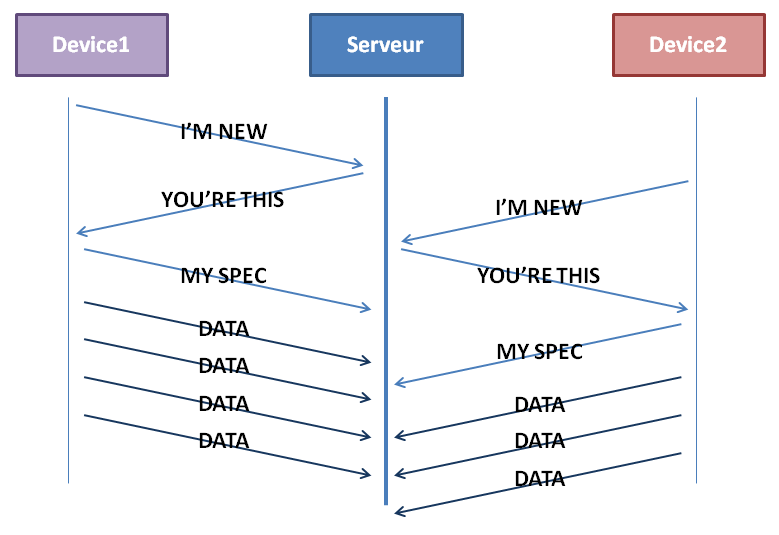
\includegraphics[width=\textwidth]{communication_example}
	\vspace{1cm}
	
	\paragraph{}
	J'ai aussi développé la partie "device" qui fait le lien entre la partie "sensor" et "communicator". Cette partie est lancée au démarrage des RPi et permet au "device" de commencer son fonctionnement.
	
	\paragraph{}
	Aussi, j'ai réalisé la partie de génération du son dans le "server". Ainsi, ce dernier peut aller chercher la dernière configuration disponible dans la base de données, retracer la structure en arbre ayant pour racine la sortie du son et générer à partir de là des portions de son de 50ms (intervalle minimal pour pouvoir avoir une période complète de la plus basse fréquence audible). Il est donc doté d'une partie permettant la lecture de son et d'une partie permettant la génération de son. De plus, une interface simple est disponible pour créer des "boxes" qui permettent de prendre un(des) son(s) ou une(des) valeur(s) et de les traiter. Chaque "box" représente un nœud de l'arbre.
	
	\paragraph{}
	Voici un exemple de configuration ainsi que son schéma fonctionnel :\\
	
	\vspace{1cm}
	\noindent
	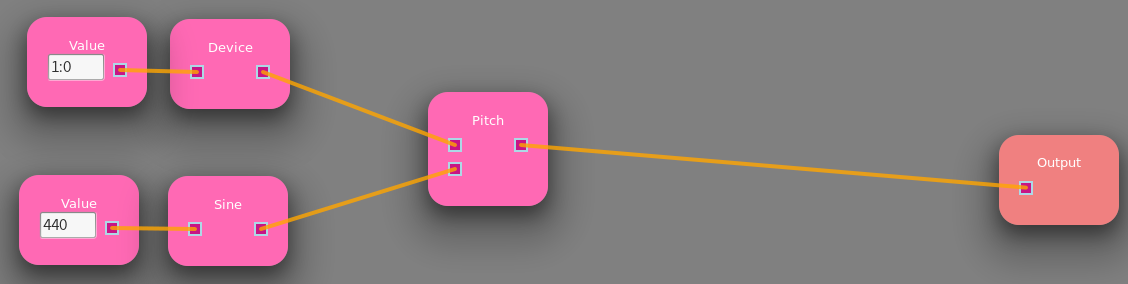
\includegraphics[width=\textwidth]{config_sheme}
	
	\vspace{1cm}
	\noindent
	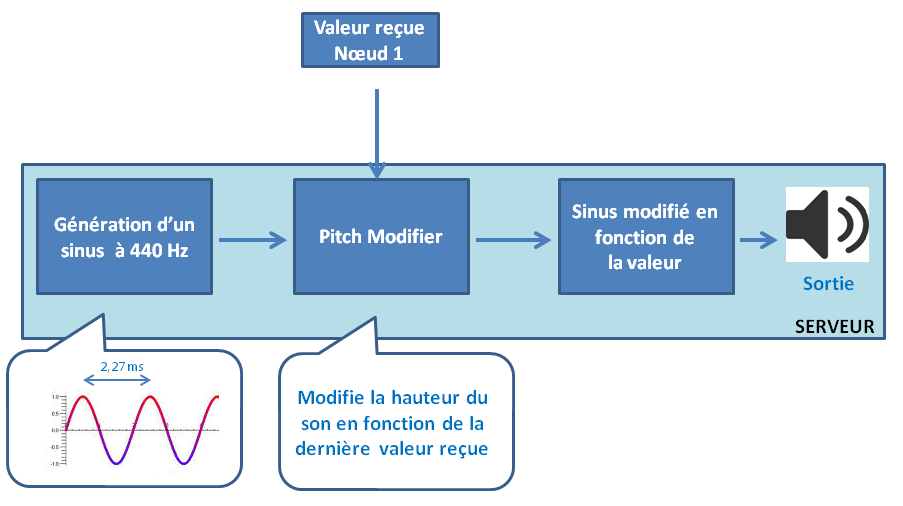
\includegraphics[width=\textwidth]{config_example}
	\vspace{1cm}
	
	\subsection{Rendu final}
	Afin de ne pas trop entrer dans le détail, voici une explication simplifiée du fonctionnement du logiciel. Tout d'abord,  le serveur Web \textit{LAMP} et le "server" doivent être mis en marche. 
	
	Ensuite, l'utilisateur peut allumer les différentes "devices". Il va maintenant pouvoir configurer le \textit{server} via l'interface Web.
	
	Dès que le "server" détecte une configuration fonctionnelle, il va l'appliquer et générer le son. Le "device" dès son allumage envoie des données au "server" qui toute les 50ms va générer du son en fonction de ces dernières et de la configuration.
	
	Enfin, le son est émis et peut être entendu.
	\subsection{Évolution}
	Le projet même si fonctionnel, est largement améliorable. En effet, tout l'intérêt de ce projet est qu'il est extrêmement modulaire et très facilement améliorable. De plus, de nouveaux "devices" peuvent être implémentés en quelques lignes et de nouveau modificateurs de son pourraient être aisément ajoutés. Une fonctionnalité de partage de configuration sur internet pourrait être très inintéressante, ce qui permettrait en plus de pouvoir sauvegarder et restaurer une configuration. Enfin, une fonctionnalité d'import de fichier son pourrait être un point amusant.
	
	\subsection{Bilan}
	Les premiers enseignements ont été riches. Nous nous sommes lancés dans une projet intéressant mais ambitieux. Nous avons beaucoup discuté du projet en cours d'ISN, mais aussi au CDI, et de nos discussions, je pensais que nous avions tous la même vision de ce qu'il fallait faire même si nous n'avancions pas au même rythme. Je ne me suis rendu compte que tardivement qu'Estelle et Nour avaient du mal à avancer et je leur ai apporté mon support pour les aider à programmer en leur expliquant comment il fallait faire.
	
	\paragraph{}
	De plus, l'arrivée tardive du code de Nour et Estelle n'a permis de faire l'intégration de l'ensemble que tardivement, ce qui a nécessité de reprendre des parties de code déjà rédigées. C'est une partie du projet que je n'avais pas envisagé de cette façon : cela m'a pris beaucoup de temps en plus de ce qui était à faire et je pense que les outils collaboratifs auraient du être utilisés plus tôt pour échanger plus vite sur les problématiques rencontrées. Afin d'améliorer l'avancement du projet, il aurait fallu rédiger un cahier des charges détaillé dès le début du projet et peut-être travailler sur un projet moins complexe : le projet nous a séduit tous les trois, mais je crois que j'étais le seul en début de projet à bien appréhender la complexité des développements.
	
	\paragraph{}
	Il aurait été judicieux aussi de faire régulièrement des points de synchronisation avec nos développements respectifs, nos réunions étaient très utiles, mais peut-être pas assez précises et détaillées sur le contenu de nos travaux, les échanges étant principalement oraux.
	
	
	\paragraph{}
	Le bilan reste très positif, le projet fonctionne bien conformément aux objectifs que nous nous étions fixés et j'ai beaucoup appris sur le travail collaboratif. Plus globalement, j'ai discuté et travaillé ponctuellement avec plusieurs personnes dans différents projets et j'ai tiré une grande satisfaction de pouvoir donner des idées, apporter un support aux différentes équipes qui pour certaines ont quelques lignes de code que j'ai pu rédiger.
	
	\vspace{1cm}
	\noindent
	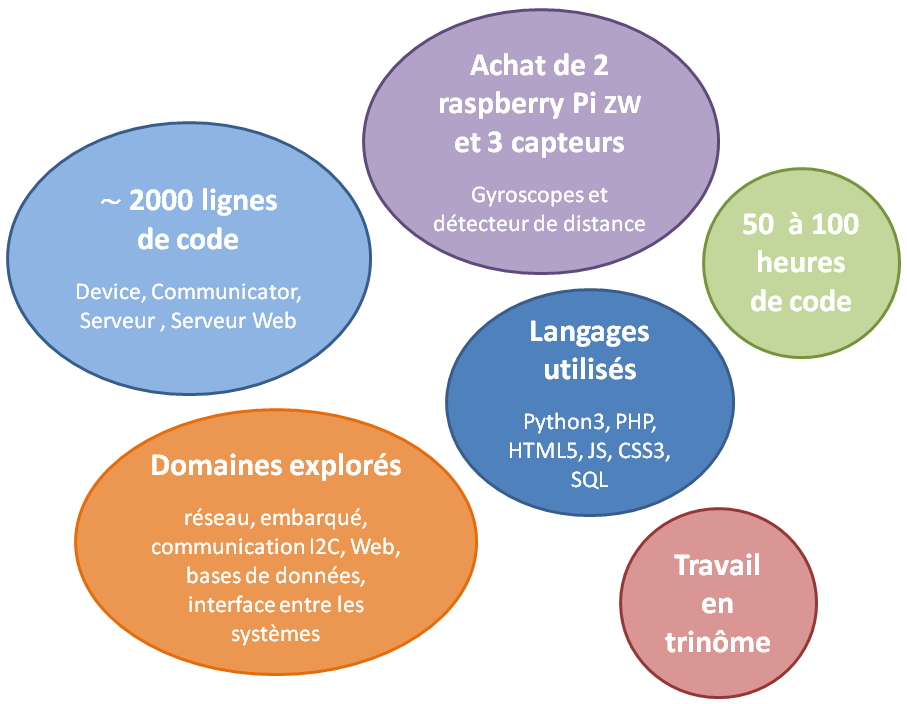
\includegraphics[width=\textwidth]{bilan}
	\vspace{1cm}
	
	\subsection{Licence}
	Ce projet est en open-source, sous la licence GPLv3, cela veut dire que n’importe qui est libre d’utiliser, de copier, de modifier et de distribuer le projet source ou dérivé, même pour de l’argent. Cependant en cas de modification, le résultat doit être placé sous la même Licence. Nous avons choisi cette licence d’abord car elle est gratuite, et ensuite car nous voulions que notre projet puisse évoluer au maximum de ses capacité et parce que nous ne sommes pas contre l’idée que quelqu’un puisse commercialiser notre projet si cela lui permet d’évoluer. C’est également dans cette optique que nous avons rendu le code disponible sur GitHub, permettant à n’importe qui de proposer des ajouts.
	\newpage
	\section*{Annexes}
	\subsection*{Music Swagger Protocol}
	\inputminted[breaklines]{text}{MusicSwaggerProtocol.txt}
	\newpage
	\subsection*{Base de donnée}
	(Certaines bases sont vides car se remplissent durant le fonctionnement)
	\begin{longtable}{|l|l|l|l|l|} 
		\caption{Content of table available\_tools} \label{tab:available_tools-data} \\\hline \multicolumn{1}{|c|}{\textbf{ID}} & \multicolumn{1}{|c|}{\textbf{inputs}} & \multicolumn{1}{|c|}{\textbf{need\_input}} & \multicolumn{1}{|c|}{\textbf{name}} & \multicolumn{1}{|c|}{\textbf{type}} \\ \hline \hline  \endfirsthead 
		\caption{Content of table available\_tools (continued)} \\ \hline \multicolumn{1}{|c|}{\textbf{ID}} & \multicolumn{1}{|c|}{\textbf{inputs}} & \multicolumn{1}{|c|}{\textbf{need\_input}} & \multicolumn{1}{|c|}{\textbf{name}} & \multicolumn{1}{|c|}{\textbf{type}} \\ \hline \hline \endhead \endfoot
		1 & 2 & 0 & Pitch & PITCH \\ \hline 
		2 & 3 & 0 & Add & ADD \\ \hline 
		3 & 0 & 1 & Value & VALUE \\ \hline 
		4 & 1 & 0 & Device & DEVICE \\ \hline 
		5 & 1 & 0 & Sine & SINE \\ \hline 
		6 & 4 & 0 & More & MORE \\ \hline 
		7 & 4 & 0 & Less & LESS \\ \hline 
		9 & 0 & 0 & Random & RAND \\ \hline 
		10 & 2 & 0 & Multiply & MULTI \\ \hline 
		11 & 2 & 0 & Sum & SUM \\ \hline 
		12 & 2 & 0 & Doppler & DOP \\ \hline 
		13 & 2 & 0 & Ampli & AMP \\ \hline 
		14 & 2 & 0 & DIST & Distortion \\ \hline 
	\end{longtable}
	\begin{longtable}{|l|l|l|l|} 
		\caption{Content of table boxes} \label{tab:boxes-data} \\\hline \multicolumn{1}{|c|}{\textbf{ID}} & \multicolumn{1}{|c|}{\textbf{TYPE}} & \multicolumn{1}{|c|}{\textbf{BOX\_ID}} & \multicolumn{1}{|c|}{\textbf{SPEC\_PARAM}} \\ \hline \hline  \endfirsthead 
		\caption{Content of table boxes (continued)} \\ \hline \multicolumn{1}{|c|}{\textbf{ID}} & \multicolumn{1}{|c|}{\textbf{TYPE}} & \multicolumn{1}{|c|}{\textbf{BOX\_ID}} & \multicolumn{1}{|c|}{\textbf{SPEC\_PARAM}} \\ \hline \hline \endhead \endfoot
	\end{longtable}
	
	%
	% Data: connections
	%
	\begin{longtable}{|l|l|l|l|} 
		\caption{Content of table connections} \label{tab:connections-data} \\\hline \multicolumn{1}{|c|}{\textbf{ID}} & \multicolumn{1}{|c|}{\textbf{GUID}} & \multicolumn{1}{|c|}{\textbf{CUID}} & \multicolumn{1}{|c|}{\textbf{inited}} \\ \hline \hline  \endfirsthead 
		\caption{Content of table connections (continued)} \\ \hline \multicolumn{1}{|c|}{\textbf{ID}} & \multicolumn{1}{|c|}{\textbf{GUID}} & \multicolumn{1}{|c|}{\textbf{CUID}} & \multicolumn{1}{|c|}{\textbf{inited}} \\ \hline \hline \endhead \endfoot
	\end{longtable}
	
	%
	% Data: links
	%
	\begin{longtable}{|l|l|l|l|} 
		\caption{Content of table links} \label{tab:links-data} \\\hline \multicolumn{1}{|c|}{\textbf{ID}} & \multicolumn{1}{|c|}{\textbf{FROM\_B}} & \multicolumn{1}{|c|}{\textbf{TO\_B}} & \multicolumn{1}{|c|}{\textbf{WHERE\_L}} \\ \hline \hline  \endfirsthead 
		\caption{Content of table links (continued)} \\ \hline \multicolumn{1}{|c|}{\textbf{ID}} & \multicolumn{1}{|c|}{\textbf{FROM\_B}} & \multicolumn{1}{|c|}{\textbf{TO\_B}} & \multicolumn{1}{|c|}{\textbf{WHERE\_L}} \\ \hline \hline \endhead \endfoot
	\end{longtable}
	%
	% Data: specifications
	%
	\begin{longtable}{|l|l|l|l|l|} 
		\caption{Content of table specifications} \label{tab:specifications-data} \\\hline \multicolumn{1}{|c|}{\textbf{ID}} & \multicolumn{1}{|c|}{\textbf{numchan}} & \multicolumn{1}{|c|}{\textbf{name}} & \multicolumn{1}{|c|}{\textbf{description}} & \multicolumn{1}{|c|}{\textbf{CUID}} \\ \hline \hline  \endfirsthead 
		\caption{Content of table specifications (continued)} \\ \hline \multicolumn{1}{|c|}{\textbf{ID}} & \multicolumn{1}{|c|}{\textbf{numchan}} & \multicolumn{1}{|c|}{\textbf{name}} & \multicolumn{1}{|c|}{\textbf{description}} & \multicolumn{1}{|c|}{\textbf{CUID}} \\ \hline \hline \endhead \endfoot
	\end{longtable}
	
	%
	% Data: update_number
	%
	\begin{longtable}{|l|} 
		\caption{Content of table update\_number} \label{tab:update_number-data} \\\hline \multicolumn{1}{|c|}{\textbf{ID}} \\ \hline \hline  \endfirsthead 
		\caption{Content of table update\_number (continued)} \\ \hline \multicolumn{1}{|c|}{\textbf{ID}} \\ \hline \hline \endhead \endfoot
	\end{longtable}
	\subsection*{device.py}
	\inputminted[breaklines,linenos]{python}{device.py}
	
	\subsection*{GitHub}
	(Tout le code ne peut pas être disponible en annexe dans un souci de gâchis de papier et de lisibilité.)
	\begin{itemize}
		\item[\url{http://github.com/TheMusicSwagger/Device}] La partie "device" du projet
		\item[\url{http://github.com/TheMusicSwagger/Server}] La partie "server" du projet
		\item[\url{http://github.com/TheMusicSwagger/Communicator}] La partie "communicator" du projet
		\item[\url{http://github.com/TheMusicSwagger/Documentation}] La documentation du projet
		
	\end{itemize}
\end{document}
